%%%%%
%%%%%  Use LUALATEX, not LATEX.
%%%%%
%%%%
\documentclass[]{VUMIFTemplateClass}

\usepackage{indentfirst}
\usepackage{amsmath, amsthm, amssymb, amsfonts}
\usepackage{mathtools}
\usepackage{physics}
\usepackage{graphicx}
\usepackage{verbatim}
\usepackage[hidelinks]{hyperref}
\usepackage{color,algorithm,algorithmic}
\usepackage[nottoc]{tocbibind}
\usepackage{tocloft}
\usepackage{booktabs}
\usepackage{multirow}
\usepackage{caption}
\usepackage{tikz}
\usetikzlibrary{shapes,arrows,positioning}

\usepackage{titlesec}
\newcommand{\sectionbreak}{\clearpage}

\makeatletter
\renewcommand{\fnum@algorithm}{\thealgorithm}
\makeatother
\renewcommand\thealgorithm{\arabic{algorithm} algorithm}

\usepackage{biblatex}
\bibliography{bibliografija}
%% to change the numbering (numeric or alphabetic) of bibliographic sources, make the change in VUMIFTemplateClass.cls, line 139

% Author's MACROS
\newcommand{\EE}{\mathbb{E}\,} % Mean
\newcommand{\ee}{{\mathrm e}}  % nice exponent
\newcommand{\RR}{\mathbb{R}}

\studyprogramme{Data Science}
\worktype{Master's thesis}
\worktitle{Data Selection Strategies for Multi-Speaker Text-to-Speech Synthesis in Lithuanian}
\secondworktitle{Work Title in Lithuanian}
\workauthor{Aleksandr Jan Smoliakov}

\supervisor{Dr.~Gerda Ana Melnik-Leroy}
\reviewer{pedagogical/scientific title Name Surname}
\scientificadvisor{Dr.~Gražina Korvel}

\begin{document}
\selectlanguage{english}

\onehalfspacing
\input{TitlePage}

% %% TODO Acknowledgements Section
% \sectionnonumnocontent{Acknowledgements}
% The author is thankful the Information Technology Research Center, Faculty of Mathematics and Informatics, Vilnius University, for providing the High-Performance Computing (HPC) resources for this research.
% %%
% %%
% %%      If you have used IT resources (CPU-h, GPU-h, other IT resources) provided by MIF for your thesis research, please leave the acknowledgement; if you have not, you can delete it.
% %%
% %%

% You can also add here acknowledgements for various other things, such as your supervisor, university, company, etc.

\singlespacing
\selectlanguage{english}

% list of figures, delete if not needed
\listoffigures

% list of tables, delete if not needed
\listoftables

% Table of contents
\tableofcontents
\onehalfspacing

%%%%%%%%%%%%%%%%%%%%%%%%%%%%%%%%%%%%%%%%%%%%%%%%%%%%%%%%%%%%%%%%%%%%%%%%%%%%%%%%
%% Introduction
%%%%%%%%%%%%%%%%%%%%%%%%%%%%%%%%%%%%%%%%%%%%%%%%%%%%%%%%%%%%%%%%%%%%%%%%%%%%%%%%
\sectionnonum{Introduction}

The goal of creating machines that can speak like humans has captivated
researchers for centuries. One of the earliest known attempts dates back to the
18th century, with Wolfgang von Kempelen's mechanical ``speaking
machine''~\cite{dudley1950speaking} that utilized a bellows-driven lung and
physical models of the tongue and lips to produce rudimentary speech sounds.

Over the centuries, understanding of human speech and advancements in
technology have driven significant progress in this field. Today's
state-of-the-art Text-to-Speech (TTS) systems, dominated by end-to-end (E2E)
neural models, have achieved highly natural speech with unprecedented acoustic
quality. Notably, these E2E systems have unified the entire synthesis process
into one or two neural networks, learning to map text inputs (graphemes or
phonemes) directly to audio outputs, and eliminating the need for complex
multi-stage pipelines.

These advancements have transformed TTS from a niche area of academic curiosity
to become essential tools in daily life. High-quality speech synthesis now
powers popular virtual assistants~\cite{hoy2018alexa} and navigation systems,
serving as a primary interface for human-computer interaction. More
importantly, it plays a critical role in accessibility, enabling screen readers
for the visually impaired~\cite{isewon2014design}, providing a voice for the
non-verbal, and democratizing access to digital
information~\cite{taylor2009text}.

However, the transition to deep learning techniques has introduced a new
dependency: data. While modern neural TTS models are capable of producing
remarkably natural speech, they are inherently ``data-hungry''. This poses a
significant challenge for low-resource languages, where large, high-quality
single-speaker datasets are often unavailable.

Training high-quality TTS models typically requires large amounts of annotated
speech data. The common recommendation is to use at least 10 to 20~hours of
recorded speech from a single speaker to achieve good synthesis quality.

The majority of existing research and commercial TTS systems focus on
high-resource languages like English, where large single-speaker datasets
(e.g., LJSpeech~\cite{ljspeech17}, VCTK~\cite{veaux2019cstr}) are readily
available. However, less-resourced languages, such as Lithuanian, often lack
such extensive datasets.

Liepa~2~\cite{liepa2project} is a Lithuanian speech corpus, released in 2020,
that contains 1000~hours of annotated speech; however, this data is distributed
across 2621~speakers, with most speakers contributing under 20~minutes each.
The top speaker has only around 2.5~hours of recorded speech, well below the
standard recommendation for single-speaker TTS training.

Having such a fragmented dataset presents a distinct engineering challenge.
While multi-speaker TTS models can leverage transfer learning to improve
quality with limited data, training on the entire 1000-hour corpus is a
time-consuming and computationally expensive process, especially in the scope
of a master's thesis. As a result, a subset of the data must be selected. This
necessitates a choice between two competing strategies under a fixed
computational budget: prioritizing \textbf{breadth} (many speakers with little
data each) or \textbf{depth} (fewer speakers with more data each).
Consequently, the question that arises is: what is the optimal strategy for
sampling multi-speaker data to maximize synthesis quality? The hypothesis is
that the depth is a more critical factor, and a minimum amount of data per
speaker is required to achieve stable convergence and high-quality synthesis.

This thesis investigates the optimal data selection strategy for training
Lithuanian multi-speaker TTS models under a fixed data budget. It aims to
answer the following research questions:

\begin{enumerate}
      \item How does the trade-off between dataset breadth (number of speakers) and depth
            (duration per speaker) affect the synthesis quality and convergence stability
            of multi-speaker TTS models?
      \item How do autoregressive (Tacotron~2) and non-autoregressive (Glow-TTS)
            architectures compare in their ability to handle data sparsity (i.e., speakers
            with under 10 minutes of data)?
      \item What is the most effective sampling strategy for the Liepa~2 corpus to maximize
            the naturalness of synthesized Lithuanian speech?
\end{enumerate}

To answer these questions, the following research objectives are defined:

\begin{itemize}
      \item Preprocess the Liepa~2 corpus and create three distinct training subsets (with
            30, 60, 180 speakers) that maintain a constant total duration of 22.5 hours but
            vary in speaker distribution.
      \item Train two distinct acoustic model architectures, Tacotron~2 (with Dynamic
            Convolutional Attention) and Glow-TTS, on each of the created subsets.
      \item Implement a text processing pipeline capable of handling Lithuanian
            accentuation and grapheme-based input.
      \item Evaluate the models using objective metrics (MCD, F0~RMSE) and conduct a
            subjective Mean Opinion Score listening test with native Lithuanian speakers to
            assess naturalness.
\end{itemize}

In this study, the scope is exclusively focused on the Lithuanian language and
the Liepa~2 speech corpus. It investigates a fixed total training data size of
22.5~hours to simulate a realistic resource budget. The models are limited to
Tacotron~2 with DCA and Glow-TTS architectures within the Coqui TTS framework,
and a pre-trained HiFi-GAN vocoder is used to isolate the performance of the
acoustic models.

In terms of limitations, the findings regarding the specific numeric trade-offs
may not generalize perfectly to other languages with different features or
datasets with different recording conditions, or different TTS architectures.
The 22.5-hour training data size is a practical constraint and may not reflect
performance at larger scales. Additionally, the study focuses on read speech
--- spontaneous speech synthesis is outside the scope of this work.

The remainder of this thesis is organized as follows: \textbf{Literature
      review} presents a literature review of relevant concepts in digital signal
processing, neural TTS architectures, and the specific challenges of Lithuanian
TTS\@. \textbf{Methodology} describes the data selection, model configurations,
and the experimental design. \textbf{Results} presents the findings of the
objective and subjective synthesis quality evaluations, analyzing the failure
modes of the models. Finally, \textbf{Conclusion} summarizes the key findings
and offers potential recommendations for future research directions in
low-resource TTS synthesis.

%%%%%%%%%%%%%%%%%%%%%%%%%%%%%%%%%%%%%%%%%%%%%%%%%%%%%%%%%%%%%%%%%%%%%%%%%%%%%%%%
%% Literature review
%%%%%%%%%%%%%%%%%%%%%%%%%%%%%%%%%%%%%%%%%%%%%%%%%%%%%%%%%%%%%%%%%%%%%%%%%%%%%%%%
\section{Literature review}

\subsection{Digital representation of audio}

Speech, or sound in general, is a continuous pressure wave that propagates
through a medium, such as air. The key properties of sound waves include
frequency (pitch), amplitude (loudness), and phase.

Converting continuous sound waves into a digital format suitable for computer
processing involves two main steps: sampling and quantization.

Sampling is the process of measuring the amplitude of the sound wave at regular
time intervals. The rate at which these samples are taken is called the
sampling rate. According to the Nyquist-Shannon~\cite{shannon1949communication}
sampling theorem, accurate reconstruction of a continuous signal requires a
sampling rate that is strictly greater than twice the highest frequency present
in the signal. Frequencies in the range between 300~Hz and 3400~Hz contribute
most to human speech intelligibility and
recognition~\cite{jothilakshmi2016large}. In text-to-speech applications,
common sampling rates for audio are 22.05~kHz and 24~kHz, which can capture
frequencies up to approximately 11~kHz and 12~kHz, respectively.

Quantization (also known as bit depth) is the mapping of continuous amplitude
values to discrete levels for digital representation, which determines the
precision of the representation. Common bit depths for audio are 16-bit and
24-bit formats. A visual representation of both sampling and quantization is
provided in~\ref{fig:sampling}

\begin{figure}[ht]
      \centering
      \includegraphics[width=0.8\textwidth]{figures/sampling_quantization.pdf}
      \caption[Visual representation of Analog-to-Digital conversion]{Visual representation of Analog-to-Digital conversion. The continuous grey line represents the analog signal. The vertical lines represent the \textbf{sampling rate} (time intervals), and the horizontal grid lines represent \textbf{quantization levels} (bit depth).}\label{fig:sampling}
\end{figure}

Pre-emphasis is a high-frequency filtering technique applied to audio signals
before further processing. Natural speech signals tend to have more energy in
the lower frequencies, with a gradual drop-off towards higher frequencies
(typically around -6~dB per octave). Pre-emphasis compensates for this spectral
tilt by boosting high frequencies using a first-order high-pass filter, which
is defined as:

\begin{equation}
      y[n] = x[n] - \alpha x[n-1]
\end{equation}

where \( y[n] \) is the pre-emphasized signal, \( x[n] \) is the original
signal, \( \alpha \) is the pre-emphasis coefficient (typically between 0.9 and
1.0, and often set to 0.97), and \( n \) is the sample index.

This transformation balances the frequency spectrum, improving the
signal-to-noise ratio for higher frequencies and preventing the model from
optimizing only for low-frequency components.

\subsection{Time-Frequency Analysis}

\subsubsection{Fourier Transform}

Fourier Transform (FT) is a mathematical technique that transforms a
time-domain signal (such as an audio waveform) into its frequency-domain
representation. The signal is decomposed into a sum of sine and cosine waves at
various frequencies, each with a specific amplitude and phase. This allows us
to analyze the frequency content of the signal.

Short-Time Fourier Transform (STFT)~\cite{gabor1946theory} extends the FT by
applying it to short, overlapping segments (frames) of the signal. This
transformation provides a time-frequency representation, showing how the
frequency content of the signal changes over time.

In TTS applications, the STFT is computed by dividing the audio signal into
short frames (usually, 20--50~ms) with a certain overlap (usually, 50--75\%)
between frames, windowed by a Hamming or Hann function to reduce the spectral
leakage.

\subsubsection{Spectrogram and Mel-spectrogram}

The spectrogram is a visual representation of the STFT, displaying frequency on
the vertical axis, time on the horizontal axis, and amplitude represented by
the color intensity.

However, the human ear does not perceive frequencies linearly --- it is more
sensitive to lower frequencies than higher ones. To mimic this perceptual
characteristic, the Mel scale~\cite{stevens1937scale} maps linear frequency \(
f \) (in Hz) to a perceptual scale \( m \) (in Mels) using the following
formula:

\begin{equation}
      m = 2595 \cdot \log_{10}\left(1 + \frac{f}{700}\right)
\end{equation}

Mel-spectrograms are computed by applying a Mel filterbank of overlapping
triangular filters (or kernels) to the magnitude spectrogram obtained from the
STFT\@. This results in a compressed representation of the audio signal that
aligns more closely with human auditory perception. Such Mel-spectrograms are
commonly used as input features for modern TTS systems. The differences between
the raw waveform, the standard spectrogram, and the Mel-spectrogram are
illustrated in~\ref{fig:waveform_spectrograms} Note how the Mel-spectrogram has
a higher resolution in the lower frequencies, where the majority of the speech
energy is concentrated.

\begin{figure}[ht]
      \centering
      \includegraphics[width=0.8\textwidth]{figures/waveform_spectrograms.pdf}
      \caption[Raw waveform, Spectrogram, and Mel-spectrogram]{Raw audio waveform (top), its spectrogram (middle), and Mel-spectrogram (bottom) representations for the utterance ``Štai ir visas mano bendravimas su vaiku''.}\label{fig:waveform_spectrograms}
\end{figure}

\subsection{Linguistic Representation (Text Processing)}

In TTS systems, the input text must be pre-processed and converted into a
suitable linguistic representation that the synthesis model can use. The main
goal is to map the raw sentences into a sequence of symbols that can be more
closely mapped to the acoustic features of speech.

Although theoretically an end-to-end TTS model could learn to map raw text
directly to audio, in practice, pre-processing the text makes the model
convergence easier and improves the quality of the synthesized speech.

This process typically involves several steps, such as text normalization,
grapheme-to-phoneme conversion, and possibly prosody prediction.

\subsubsection{Text normalization}

Text normalization~\cite{sproat2001normalization} is the process of converting
raw written text with non-standard words into a more standardized ``spoken''
form. Typical steps include expanding abbreviations (e.g., expanding ``Dr.'' to
``Doctor''), punctuation removal, number normalization (e.g., converting
``123'' to ``one hundred twenty-three''), and lowercasing.

As an example, the input text ``Dr.\ Smith has 2 cats.'' could be normalized to
``doctor smith has two cats''.

Text normalization helps reduce the variability and complexity in the input
text, decreases the number of unique symbols, and removes the ambiguities that
could confuse the TTS model. The resulting normalized text is not only easier
for the model to process, but can also be further converted into phonemes,
which provide an even closer representation of the spoken language.

\subsubsection{Graphemes vs. Phonemes}

Text-to-speech systems use a discrete input representation derived from text,
generally divided into grapheme-based or phoneme-based sequences.

Grapheme-based models ingest raw character sequences (orthography). This
approach simplifies the inference pipeline by eliminating the dependency on
external grapheme-to-phoneme (G2P) converters. However, it forces the model to
implicitly learn pronunciation rules from data, which can be a significant
challenge for languages with complex orthographies or inconsistent
grapheme-to-phoneme mappings (e.g., ``read'' /riːd/ vs.\ ``read'' /rɛd/,
depending on the tense).

In contrast, the phoneme-based approach uses a phonetic transcription of the
text, typically in the International Phonetic Alphabet (IPA) or ARPABET form.
By resolving pronunciation ambiguities prior to training, phonemes provide a
more direct mapping to acoustic features, simplifying the model's task of
learning alignment. The downside is that this approach requires an external G2P
conversion step~\cite{bisani2008joint}. Additionally, errors in the G2P
conversion can propagate to the TTS model, affecting the quality of the
synthesized speech.

There is another approach that augments the grapheme-based representation with
explicit lexical stress markers or diacritics (e.g., tilde, acute, grave
accents). This intermediate method helps the model disambiguate pronunciation
of homographs and easier learn prosodic patterns without requiring a full
phonetic transcription, particularly in languages where stress placement alters
meaning.

\subsubsection{Specific challenges in Lithuanian}

Lithuanian is a Baltic language with a rich inflectional morphology and complex
prosodic structure. It is a pitch-accent language with free stress, meaning the
stress can fall on any syllable in a word, and can change the position
depending on the grammatical form.

Challenges in Lithuanian TTS synthesis include:

\begin{itemize}
      \item \textbf{High out-of-vocabulary word rate:} Due to extensive word inflection, the number of unique word forms is significantly higher than in English. This leads to data sparsity issues where many valid word forms may not appear in the training set.
      \item \textbf{Ambiguity without accentuation:} Typically, stress marks are omitted in written Lithuanian. However, stress position and tone (acute, circumflex, or short) determine the meaning of monographic words. Examples are shown in~\ref{tab:lithuanian_ambiguity} A grapheme-based model with accentuation marks has been shown to improve synthesis quality in Lithuanian~\cite{kasparaitis2023investigation}.
\end{itemize}

\begin{table}[ht]
      \centering
      \begin{tabular}{lcc}
            \toprule
            \textbf{Word}          & \textbf{Accentuation}       & \textbf{Meaning}      \\
            \midrule
            \multirow{2}{*}{Antis} & \textit{ántis} (Acute)      & A duck (noun)         \\
                                   & \textit{añtis} (Circumflex) & Bosom/Chest (noun)    \\
            \midrule
            \multirow{2}{*}{Kasa}  & \textit{kãsa} (Circumflex)  & He/she digs (verb)    \\
                                   & \textit{kasà} (Short)       & Braid/Pancreas (noun) \\
            \bottomrule
      \end{tabular}
      \caption[Lithuanian homographs with accentuation ambiguity]{Examples of Lithuanian homographs where accentuation determines meaning. A grapheme-only model cannot distinguish these without context or explicit stress marks.}\label{tab:lithuanian_ambiguity}
\end{table}

To overcome these challenges, tools like
\textbf{Kirčiuoklis}~\cite{kirciuoklis} (Vytautas Magnus University) are often
employed in the text normalization pipeline. Kirčiuoklis automatically assigns
stress marks to raw text. One weakness of Kirčiuoklis is that it relies on
simple word-dictionary based lookup, which does not take into account the
context of the word. Thus, it suggests multiple possible accentuation variants
for homographs, leaving it up to the user to select the correct one.

In the absence of a high-quality, context-aware G2P converter for Lithuanian,
this thesis will focus on grapheme-based TTS synthesis with accentuation marks
provided by Kirčiuoklis. In cases where Kirčiuoklis suggests multiple
accentuation variants for a word, no stress marks will be added, leaving the
TTS model to infer the correct prosody from context.

\subsection{Embeddings and Representation Learning}

\subsubsection{The Concept of Embeddings}

In machine learning, embeddings are dense vector representations of discrete
entities (such as words, characters, or speakers) to a high-dimensional
continuous vector space. Unlike one-hot encodings, which are sparse and highly
dimensional, embeddings provide a dense, lower-dimensional representation that
captures semantic relationships between underlying entities. For instance, in
word embeddings, similar words tend to have more similar (correlated) vector
representations, while dissimilar words map to more distant points in the
vector space~\cite{mikolov2013efficient}.

\subsubsection{Text Embeddings}

The ``Encoder'' part of a TTS model is responsible for converting a sequence of
input symbols (characters or phonemes) into a sequence of feature vectors.
Usually, this is done using an embedding layer, which maps each ``categorical''
input symbol to a learnable fixed-size vector representation. During training,
these embeddings are learned jointly with the rest of the TTS model.

\subsection{Text-to-speech synthesis}

Text-to-Speech (TTS) synthesis, also known as speech synthesis, is the process
of converting written text into human-like spoken words. Nowadays TTS is a key
technology in numerous applications, including virtual assistants,
accessibility tools, and language learning platforms.

The \textit{one-to-many} nature of the mapping from text to speech adds
presents a significant challenge, where a single text input can map to multiple
speech outputs with a variety of speaking styles, emotions, and prosodic
variations~\cite{jawaid2024style}. Thus, TTS is inherently a
\textit{large-scale inverse problem}~\cite{wang2017tacotron} --- reconstructing
the original waveform from incomplete data (text) requires inferring missing
information.

\subsubsection{Traditional TTS approaches}

Early attempts at artificial speech synthesis evolved from the first mechanical
devices in the 18th century to electronic systems. Wolfgang von Kempelen's
mechanical speaking machine~\cite{dudley1950speaking} demonstrated basic
phoneme, and later short phrase production using a physical model of the vocal
tract. In 1939, Homer Dudley's invention of the
Voder~\cite{dudley1939synthetic} became the first electronic speech synthesizer
that could produce intelligible speech through operator-controlled acoustic
parameters, establishing the foundation for modern electronic synthesis
methods.

In the decades that followed, two main approaches for speech synthesis emerged:
concatenative synthesis and parametric synthesis.

\subsubsection{Concatenative synthesis}

The concatenative synthesis approach~\cite{hunt1996unit} synthesizes speech by
piecing together pre-recorded segments of human speech. This method involves
several steps. First, it requires pre-recording a large database of speech
segments spoken by a human voice actor in pristine, highly controlled studio
conditions to ensure consistent audio quality and minimize background noise.
Each segment is labeled and indexed based on its phonetic and prosodic
properties.

During synthesis, the system breaks down the input text into short linguistic
units (such as phonemes or syllables) using a text analysis module. Then, it
queries the speech database to find the best-matching segments for each unit
using selection cost functions~\cite{black1996optimising}. The retrieved
segments are blended and concatenated to form a continuous speech waveform.
Finally, the system uses signal processing techniques to smooth the transitions
between segments and adjust pitch and duration to match the desired output
characteristics.

Although concatenative synthesis is a fast method capable of producing
high-quality speech, its performance is heavily dependent on the size and
quality of the underlying speech corpus~\cite{kuligowska2018speech}. A
significant limitation is that the system fails to maintain naturalness when
the required speech segments are not present in the database. However, even the
largest corpora cannot cover all variants of contextual speech segments. When
the system has to synthesize out-of-database segments, the final audio suffers
from audible continuity distortions at the concatenation
points~\cite{black1996optimising}. The segments may not blend smoothly due to
differences in pitch, duration, and timbre --- as a result, stringing
disjointed segments together does not capture the natural rhythm and intonation
patterns of connected speech.

The creation of a comprehensive corpus for such a purpose is costly and
time-consuming. Improving a concatenative system requires language-specific
expertise to design and update the corpus with good-quality, well-pronounced
word units~\cite{kuligowska2018speech}. These rigid requirements are especially
challenging for languages with rich morphology, and especially for low-resource
languages like Lithuanian.

\subsubsection{Parametric synthesis}

In contrast, statistical parametric speech synthesis~\cite{zen2009statistical}
(SPSS) uses statistical models, typically Hidden Markov Models
(HMMs)~\cite{tokuda2013speech}, to generate the parameters that control a
speech waveform.

The workflow has two distinct stages: training and
synthesis~\cite{zen2009statistical}. In the training stage, the model analyzes
a large corpus of recorded speech to learn the relationship between linguistic
features (e.g., phonemes, prosody) and the statistical distributions of
acoustic features (e.g., spectral envelope, fundamental frequency). In the
synthesis stage, the system converts input text into a sequence of linguistic
features, the trained model predicts the corresponding acoustic parameters, and
finally the speech waveform is reconstructed based on these predictions.

Compared to concatenative synthesis, the statistical approach allows for more
flexibility and control over the speech synthesis process, enabling the
generation of a variety of voices, speaking styles, and emotions.

However, HMM-based synthesis~\cite{tokuda2013speech} had a persistent problem:
the statistical averaging built into the models tended to over-smooth the
acoustic features, creating the characteristic ``buzzy'' or ``muffled'' sound
that lacked the sharpness and detail of natural human speech. In general,
well-tuned concatenative synthesis produced higher-quality speech than the best
parametric methods.

\subsection{Deep learning for TTS}

The limitations of complex, multi-stage pipelines motivated the creation of the
E2E model. E2E systems learn the entire speech synthesis process --- from input
text directly to acoustic output --- using a single neural network. This
approach promised to eliminate the need for hand-crafted pipelines that were
difficult to design, required extensive expertise, and suffered from errors
that accumulated across multiple components. By learning directly from
text-audio pairs, E2E models showed they could produce speech with higher
naturalness and expressiveness than previous methods, representing a
significant leap in TTS technology.

Although deep learning TTS models are more robust to variations in data quality
compared to concatenative approaches, they are essentially ``data-hungry''
systems that require large amounts of training data to achieve optimal
performance. Extrapolating from results in language modeling, it is observed
that model performance follows general scaling laws~\cite{kaplan2020scaling},
improving as the amount of training data increases.

However, in the context of multi-speaker synthesis, there is a trade-off
between the breadth of the data (number of distinct speakers) and the depth of
the data (duration of audio per speaker). In theory, training on a dataset with
a massive number of speakers, even with limited data per speaker, may allow the
model to learn a more generalized latent space of voice characteristics. This
high variance in the training data could act as a form of regularization,
preventing overfitting to noise and idiosyncrasies of individual speakers. In
contrast, datasets with fewer speakers but high duration per speaker allow the
model to capture fine-grained prosodic details specific to those voices,
potentially achieving higher stability but lower generalization capabilities.

\subsubsection{Feedforward neural networks}

Feedforward Neural Networks (FNNs) are the simplest type of artificial neural
networks, consisting of layers of interconnected nodes (neurons) where
information flows in one direction --- from the input, through hidden layers,
to the output. While FNNs can be useful for basic regression or classification
tasks, they lack the memory and context-awareness needed for processing
sequential data like text and speech. Therefore, FNNs are not suitable for
modelling TTS tasks that require understanding of temporal dependencies.

\subsubsection{Encoder-Decoder architectures}

The Encoder-Decoder architecture is a neural network architecture consisting of
two components, namely an encoder and a decoder. The encoder processes the
input data and compresses it into a high-dimensional latent representation.
This vector captures the meaningful features of the input. The decoder uses
this latent representation as context to generate the final output. This
architecture is commonly used in sequence-to-sequence tasks, such as machine
translation (text-to-text) and text-to-speech synthesis (text-to-audio frames).

\subsubsection{Sequence-to-Sequence models and Tacotron~2}

A common approach in modern neural TTS is the sequence-to-sequence (seq2seq)
framework~\cite{sutskever2014sequence}, which uses an encoder-decoder
architecture with an attention mechanism to map input (text) sequences to
output (audio) frames.

Tacotron~\cite{wang2017tacotron} and Tacotron~2~\cite{shen2018natural} are two
notable TTS models based on the sequence-to-sequence architecture. The variant
that this thesis primarily focuses on is Tacotron~2 with Dynamic Convolutional
Attention (DCA). The complete architecture of Tacotron~2 is depicted
in~\ref{fig:tacotron_arch}

This architecture has three main components:

\begin{enumerate}
      \item \textbf{Encoder:} The encoder's input is a character or phoneme sequence. A stack of convolutional layers followed by a bidirectional LSTM converts the character sequence into a high-level hidden feature representation.
      \item \textbf{Attention mechanism:} A location-sensitive attention~\cite{chorowski2015attention} mechanism learns to align the high-level text representation with the decoder steps. This alignment determines which parts of the input text should be attended to when generating each of the output audio frames.
      \item \textbf{Decoder and Post-net:} The autoregressive LSTM decoder generates a coarse Mel-spectrogram frame. This output is then passed through a convolutional \textbf{Post-net} which predicts a residual to refine the spectral details and improve reconstruction quality.
      \item \textbf{Stopnet:} A linear layer projects the LSTM decoder's output to a scalar, predicting the probability that the current frame is the ``stop token'', which halts the synthesis process. This allows the model to dynamically determine the output duration.
\end{enumerate}

The model is optimized by minimizing a combination of losses: the mean squared
error (MSE) between the predicted and ground truth Mel-spectrograms (both the
Decoder and Post-net outputs), the spectral similarity index (SSIM) loss for
improving spectral similarity, the ``guided attention'' loss to encourage
diagonal attention alignments, and the binary cross-entropy loss for the stop
token prediction.

While Tacotron~2 can generate high-quality speech, its autoregressive nature
makes inference slow, as each audio frame must be generated sequentially.
Additionally, the attention mechanism can sometimes fail, leading to issues
like skipped or repeated words in the synthesized speech.

\begin{figure}[ht]
      \centering
      % \includegraphics[width=\textwidth]{}
      \caption[Tacotron~2 architecture]{The Tacotron~2 architecture. Note the recurrent connections in the decoder and the attention mechanism aligning encoder outputs to decoder steps~\cite{shen2018natural}.}\label{fig:tacotron_arch}
\end{figure}

\subsubsection{Non-autoregressive models and Glow-TTS}

To address the slow inference speed and stability issues of autoregressive
models, non-autoregressive (parallel) models were developed.
Glow-TTS~\cite{kim2020glowtts} is a notable example of such a model that is a
notable example of such a model that applies flow-based generative models to
text-to-speech tasks.

Unlike Tacotron~2, Glow-TTS model generates the entire Mel-spectrogram in
parallel, significantly speeding up the inference. It utilizes an invertible
flow-based decoder. A key innovation of Glow-TTS is its ability to learn
alignment internally without requiring external priors (aligner), achieved
through the following components:

\begin{itemize}
      \item \textbf{Monotonic Alignment Search (MAS):} Unlike FastPitch~\cite{lancucki2020fastpitch}, which relies on external aligners to train a duration predictor, Glow-TTS treats alignment as a latent variable. It employs MAS to find the most probable monotonic path between the input text and the target Mel-spectrogram, maximizing the log-likelihood of the data.
      \item \textbf{Flow-based decoder:} The model uses a stack of normalizing flows—specifically invertible $1 \times 1$ convolutions and affine coupling layers. This decoder transforms a simple prior distribution (conditioned on the text input) into the complex distribution of Mel-spectrograms.
\end{itemize}

By utilizing the properties of flows, Glow-TTS allows for varied speech
synthesis by sampling from the latent space and manipulating the noise
temperature. Furthermore, the duration of the speech can be controlled by
modifying the predicted duration of the alignment.

The high-level architecture of Glow-TTS is shown in~\ref{fig:glow_tts_arch}

\begin{figure}[ht]
      \centering
      % \includegraphics[width=\textwidth]{figures/glow_tts_arch.pdf}
      \caption[Glow-TTS architecture]{The Glow-TTS architecture. It utilizes a Transformer-based text encoder and a flow-based decoder, connected via Monotonic Alignment Search to enable parallel Mel-spectrogram generation~\cite{kim2020glowtts}.}\label{fig:glow_tts_arch}
\end{figure}

The primary advantages of Glow-TTS over Tacotron~2 are inference speed (due to
non-autoregressive generation), robustness (the monotonic constraint prevents
skipping or repeating words), and the elimination of the need for an external
aligner during training.

\subsubsection{Other notable TTS models}

Besides Tacotron~2 and Glow-TTS, other notable TTS architectures include
\textbf{FastPitch}~\cite{lancucki2020fastpitch}, which uses a feed-forward
Transformer architecture with explicit pitch and duration predictors, and
\textbf{VITS} (Conditional Variational Autoencoder with Adversarial
Learning)~\cite{kim2021conditional}, which combines the acoustic TTS model
(Glow-TTS) with a neural vocoder (HiFi-GAN) into a single end-to-end
architecture.

\subsubsection{Neural vocoders}

\begin{figure}[ht]
      \centering
      \includegraphics[width=\textwidth]{figures/tts_pipeline.pdf}
      \caption[Text-to-Speech synthesis pipeline]{Text-to-Speech synthesis pipeline. The TTS model generates Mel-spectrograms from input text, which are then converted to raw audio waveforms by a neural vocoder.}\label{fig:tts_pipeline}
\end{figure}

As illustrated in~\ref{fig:tts_pipeline}, modern TTS systems typically employ a
two-stage pipeline: an acoustic model like Tacotron~2 and Glow-TTS generates
intermediate acoustic features (Mel-spectrograms), but do not directly produce
raw audio waveforms. Spectrograms are lossy representations that only capture
the magnitude of the sound frequency bands, discarding phase information.
Converting a lossy spectrogram into audio is a non-trivial task, as the phase
information must be estimated.

An additional component called a vocoder is required to reconstruct the raw
waveform from the Mel-spectrogram.

Traditionally, the Griffin-Lim algorithm~\cite{griffin1984signal} has been used
to iteratively estimate and reconstruct the phase information from the
magnitude spectrogram. However, this method often produces audio with
noticeable artifacts and lower quality compared to natural speech.

Modern TTS systems use neural vocoders, which are deep generative models
trained to map acoustic features to raw waveforms.
\textbf{WaveNet}~\cite{oord2016wavenet} was one of the first autoregressive
models to produce high-fidelity audio, but its sequential generation process
made it prohibitively slow for real-time applications.

To address the speed limitations, Generative Adversarial Network (GAN) based
vocoders were introduced. \textbf{HiFi-GAN}~\cite{kong2020hifi} is currently
one of the state-of-the-art neural vocoders. It consists of a Generator that
upsamples the Mel-spectrograms using transposed convolutions and a set of
Discriminators (multi-scale and multi-period discriminators) that ensure the
generated audio is indistinguishable from real human speech. HiFi-GANs are
highly efficient and capable of faster-than-real-time synthesis on consumer
hardware while maintaining high perceptual quality.

The framework used in this thesis, Coqui TTS~\cite{coqui2021}, comes with a
pre-trained HiFi-GAN v2 vocoder trained on a large multi-speaker dataset
(VCTK~\cite{veaux2019cstr}) with 110 English speakers.

The use of a vocoder trained on English data for Lithuanian synthesis is
justified by the language-agnostic nature of the phase reconstruction task.
Neural vocoders' primary function is to model the physics of human speech
production rather than linguistic features. While language-dependent phonetic
nuances exist, studies have shown that vocoders trained on large, diverse
datasets can effectively generalize to unseen speakers and
languages~\cite{lorenzo2019towards}. Therefore, this thesis will utilize the
pre-trained HiFi-GAN~v2 model for waveform generation.

This should allow the vocoder model to effectively generalize to unseen
speakers and languages, provided that the acoustic feature parameters
(including sampling rate, FFT size, Mel-filterbank limits) of the input
Mel-spectrograms match those used during the vocoder's training.

Therefore, this thesis will utilize the pre-trained HiFi-GAN v2 model for
waveform generation. The TTS models' acoustic parameters will be configured to
the exact same acoustic parameters used during the vocoder's training to ensure
compatibility.

\subsection{Multi-speaker TTS}

Multi-speaker TTS models are designed to synthesize speech in the voices of
multiple speakers. In order to achieve this, these models are indeed trained on
data from many different speakers, allowing them to learn the characteristics
of each voice and synthesize speech that sounds like a specific individual,
while still being able to generalize the shared linguistic and acoustic
patterns across speakers.

\subsubsection{Speaker embeddings}

To enable multi-speaker synthesis, TTS models require a representation of the
speaker's identity. In multi-speaker models, the network is conditioned on a
speaker embedding. The model learns a shared representation of phonetics (how
text maps to sound generally) while using an additional input --- the speaker
embedding --- to adjust the timbre and prosodic characteristics specific to a
voice.

Early successful implementations of this approach include Deep Voice
2~\cite{arik2017deep}, which demonstrated effective multi-speaker synthesis by
learning speaker-specific embeddings.

Nowadays there are several techniques for incorporating speaker embeddings into
TTS models:

\textbf{Lookup Tables (LUT):} Early multi-speaker approaches used simple, learnable embeddings
where each speaker ID is mapped to a unique vector. The vectors are initialized randomly and learned
jointly with the TTS model. While this method is straightforward
and efficient, it cannot generalize to speakers not seen during training.

\textbf{d-vectors and x-vectors:} Transfer learning
approaches~\cite{jia2019transfer} have demonstrated adapting speaker
verification models for multispeaker TTS synthesis, enabling better speaker
adaptation and higher voice quality. The general architecture of such a speaker
encoder is illustrated in~\ref{fig:speaker_encoder} A speaker encoder
model pre-trained on a massive, noisy dataset with thousands of speakers (e.g.,
the VoxCeleb dataset~\cite{nagrani2017voxceleb}) learns the general speaker
space. Its pre-trained weights are frozen and used to extract embeddings for
the TTS training data, allowing the TTS model to effectively account for
multi-speaker variation.

\begin{figure}[ht]
      \centering
      % \includegraphics[width=\textwidth]{figures/speaker_encoder_diagram.pdf}
      \caption[General architecture of a Speaker Encoder]{General architecture of a Speaker Encoder. A reference audio of arbitrary length is processed (typically by LSTM or TDNN layers) and pooled to produce a fixed-length embedding vector (e.g., d-vector) representing the speaker identity.}\label{fig:speaker_encoder}
\end{figure}

\textbf{d-vectors:} d-vectors~\cite{variani2014deep} are fixed-length speaker embeddings derived from a separate speaker verification model. A reference encoder network takes a reference audio recording of arbitrary length and compresses it into a fixed-length vector known as a d-vector, that summarizes the speaker's timbral and prosodic characteristics. These d-vectors are then provided as additional input to the TTS model, and are kept fixed during TTS training.

\textbf{x-vectors:} An evolution of d-vectors, x-vectors~\cite{snyder2018x} use a Time Delay Neural Network (TDNN) architecture to capture the temporal context more effectively. These embeddings have shown an improved ability in zero-shot TTS scenarios.

One limitation of d-vectors and x-vectors is that if the reference audio is of
poor quality or contains background noise, the resulting speaker embedding may
not accurately represent the speaker's identity, leading to degraded synthesis
quality.

% TODO How Coqui TTS handles speakers: Specifically, how speaker embeddings are
% concatenated or added to the encoder outputs to condition the synthesis on a
% specific voice identity.

\subsubsection{Challenges}

One key challenge in multi-speaker TTS is ensuring that the model can
generalize across many speakers while still maintaining high quality for each.
There is a trade-off between the \textit{breadth} of the dataset (number of
speakers) and the \textit{depth} (minutes of audio per speaker).

Standard TTS systems historically required 10 to 20 hours of recorded speech
for a single professional speaker. However, deep learning models capable of
\textit{transfer learning} can produce intelligible speech for a new speaker
with significantly less data, potentially as little as a few minutes --- if the
base model has been pre-trained on a sufficiently diverse multi-speaker
dataset.

\subsection{Evaluation metrics}

Evaluating Text-to-Speech systems is notoriously difficult because ``quality''
is a subjective metric defined by human perception. There is no single
mathematical objective function that perfectly correlates with human judgement
of naturalness and intelligibility. Therefore, TTS systems are typically
evaluated using subjective listening tests.

\subsubsection{Mean Opinion Score (MOS)}

The most standard metric for evaluating speech synthesis quality is the Mean
Opinion Score (MOS), originally derived from telecommunications quality
standards (ITU-T P.800)~\cite{itup800}.

In a MOS test, human listeners (raters) are presented with a set of synthesized
speech audio samples and asked to rate them on a 5-point Likert scale. The
standard scale for ``Naturalness'' is:

\begin{itemize}
      \item \textbf{5:} Excellent (Imperceptible difference from real speech)
      \item \textbf{4:} Good (Perceptible but not annoying)
      \item \textbf{3:} Fair (Slightly annoying)
      \item \textbf{2:} Poor (Annoying)
      \item \textbf{1:} Bad (Very annoying / Unintelligible)
\end{itemize}

The final score is the arithmetic mean of all ratings collected for a specific
TTS system. Although MOS is subjective, with a sufficient number of raters
(typically, at least 15--20), the scores tend to converge and provide a
reliable ranking between different models.

\subsubsection{Latin square design}

A major challenge in subjective listening tests is controlling for biases. If a
rater hears the same sentence produced by different TTS systems in a row, their
ratings may be influenced by the repetition (repetition effect) or by the
relative order of presentation (order effect). For instance, a ``Slightly
annoying'' sample may be rated more harshly if it follows an ``Excellent''
sample (contrast effect).

In order to mitigate these biases, a Latin square
design~\cite{williams1949experimental} is often employed for MOS tests. In this
experimental design:

\begin{enumerate}
      \item A set of test sentences (utterances) is selected.
      \item The listeners are divided into groups.
      \item The presentation is balanced such that each listener hears every test sentence
            exactly once, and every TTS system (model) exactly once per block of trials,
            but never the same sentence-system combination twice.
\end{enumerate}

\begin{figure}[ht]
      \centering
      \includegraphics[width=0.6\textwidth]{figures/latin_square_design.pdf}
      \caption[Latin square design for TTS evaluation]{Latin square design for TTS evaluation. Each listener group hears each sentence exactly once, and each TTS system exactly once per block, ensuring balanced exposure and mitigating order/repetition biases.}\label{fig:latin_square}
\end{figure}

An example Latin square design for 4 TTS systems and 4 test sentences is
illustrated in~\ref{fig:latin_square}

For a multi-speaker TTS evaluation (as is the case in this thesis), the Latin
square design ensures that the ratings reflect the quality of the model rather
than the linguistic content of the sentence or listener fatigue. By rotating
the systems and sentences across listener groups, the influence of specific
difficult sentences is averaged out across all models.

\subsection{Research gap}

While the literature demonstrates the capabilities of modern deep learning TTS
architectures like Tacotron~2 and Glow-TTS to produce highly natural-sounding
speech, several questions remain unanswered regarding their application to
low-resource, morphologically complex languages like Lithuanian.

Firstly, although neural TTS models may follow general neural model scaling
laws~\cite{kaplan2020scaling}, implying that performance improves with more
data, there is limited understanding of the optimal composition of training
data under a fixed budget. In low-resource settings, scaling up the dataset
size is not always feasible, and this may be further constrained by the
computational resources required for training large models. A critical question
is whether it is more beneficial to train on a smaller number of speakers with
more data per speaker (high depth) or a larger number of speakers with less
data per speaker (high breadth).

Current research primarily focuses on high-resource languages like English,
where the availability of large, balanced multi-speaker datasets masks the
nuances of this trade-off. For a pitch-accent language like Lithuanian, the
requirements may be different. It is hypothesized that high-diversity datasets
may help the model learn a richer representation of prosodic patterns, while
high-depth datasets may improve the model's naturalness for the target
speakers.

Secondly, most multi-speaker TTS research assumes access to large-scale
datasets with thousands of utterances per speaker. There is a lack of research
exploring how different TTS architectures (autoregressive vs.
non-autoregressive) perform when the data per speaker is scarce (e.g., under 10
minutes).

This thesis aims to fill the research gap by systematically evaluating the
efficiency of Tacotron~2 and Glow-TTS models trained on Lithuanian speech data.
By controlling the total dataset size and varying the distribution of speakers
and data per speaker, this study will provide insights into the optimal data
composition for training multi-speaker TTS models in low-resource settings.

To summarize, the key research questions this thesis seeks to answer are:

\begin{itemize}
      \item How does the trade-off between data breadth (number of speakers) and data depth
            (minutes per speaker) affect the performance of multi-speaker TTS models for
            Lithuanian?
      \item How do different TTS architectures (Tacotron~2 vs. Glow-TTS) perform under
            varying data selection strategies in low-resource settings?
\end{itemize}

The experiments will involve training models on three distinct data selection
strategies:

\begin{itemize}
      \item \textbf{High-resource per speaker:} Fewer speakers (30), but high fidelity (45 min each), total: 22.5 hours.
      \item \textbf{Balanced:} Moderate diversity (60 speakers), moderate data (22.5 min each), total: 22.5 hours.
      \item \textbf{High-diversity:} Many speakers (180), low resource (7.5 min each), total: 22.5 hours.
\end{itemize}

The extreme low-depth condition (7.5 minutes per speaker) might pose
convergence challenges for the models, especially for Tacotron~2, which relies
on learning robust attention alignment. Thus, alignment convergence and
training stability will be monitored to assess how data composition affects
model robustness.

\subsection{Summary}

This literature review has provided an overview of the theoretical foundations
required for modern Text-to-Speech synthesis. The evolution of TTS systems from
mechanical apparatuses, through concatenative and statistical methods, to
end-to-end deep learning architectures capable of generating natural-sounding
speech has been discussed.

We have reviewed the entire TTS pipeline --- from signal processing (sampling,
quantization, Fourier transforms, and Mel-spectrogram extraction), through text
normalization and representation (graphemes vs.\ phonemes), to deep learning
architectures for acoustic modeling and vocoding. The literature highlights two
architectures for acoustic modeling: the autoregressive Tacotron~2, known for
high-quality spectral output but slow inference and stability issues, and the
non-autoregressive Glow-TTS, which offers parallel generation and improved
robustness.

We have examined the challenges specific to Lithuanian TTS synthesis. Unlike
English, Lithuanian languages's high inflectional morphology leads to a large
number of unique word forms, and its prosodic system requires handling of free
stress and pitch accents, necessitating the use of tools like Kirčiuoklis for
accentuation marking.

Finally, we have reviewed the role of speaker embeddings in enabling
multi-speaker synthesis and the use of neural vocoders, specifically HiFi-GAN,
to reconstruct high-fidelity waveforms from Mel-spectrograms. Despite these
advancements, a gap remains in understanding how data diversity versus quantity
affects model performance for complex, low-resource languages --- a challenge
this thesis addresses through the experiments detailed in the following
chapters.

%%%%%%%%%%%%%%%%%%%%%%%%%%%%%%%%%%%%%%%%%%%%%%%%%%%%%%%%%%%%%%%%%%%%%%%%%%%%%%%%
%% Methodology
%%%%%%%%%%%%%%%%%%%%%%%%%%%%%%%%%%%%%%%%%%%%%%%%%%%%%%%%%%%%%%%%%%%%%%%%%%%%%%%%
\section{Methodology}

This chapter details the experimental setup, data processing pipeline, training
configurations, and evaluation protocol used to determine the optimal
composition of multi-speaker training data for Lithuanian TTS\@. The study uses
factorial design to compare the performance of two distinct architectures ---
Tacotron~2 (autoregressive) and Glow-TTS (non-autoregressive) --- under varying
degrees of data breadth and depth, while controlling for the total training
budget.

The high-level experimental workflow is illustrated in~\ref{fig:pipeline}

\begin{figure}[htbp]
      \centering
      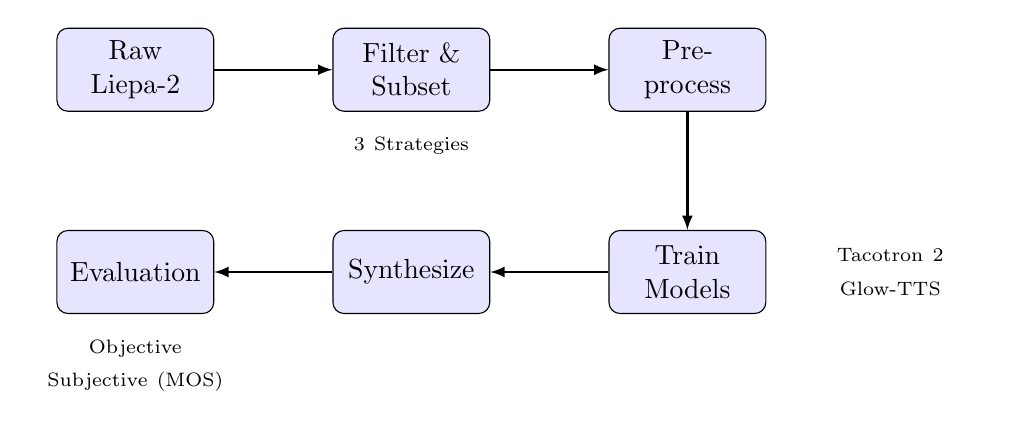
\begin{tikzpicture}[
                  node distance=1.5cm, auto,
                  block/.style={rectangle, draw, fill=blue!10, text width=5em, text centered, rounded corners, minimum height=3em},
                  line/.style={draw, -latex, thick},
                  cloud/.style={draw, ellipse, fill=red!10, node distance=2.5cm, minimum height=2em}
            ]

            % Nodes
            \node [block] (raw) {Raw Liepa-2};
            \node [block, right=of raw] (filter) {Filter \& Subset};
            \node [block, right=of filter] (preproc) {Pre-process};
            \node [block, below=of preproc] (train) {Train Models};
            \node [block, left=of train] (synth) {Synthesize};
            \node [block, left=of synth] (eval) {Evaluation};

            % Edges
            \path [line] (raw) -- (filter);
            \path [line] (filter) -- (preproc);
            \path [line] (preproc) -- (train);
            \path [line] (train) -- (synth);
            \path [line] (synth) -- (eval);

            % Labels
            \node [below=0.2cm of filter, text width=2cm, align=center] {\scriptsize 3 Strategies};
            \node [right=0.2cm of train, text width=2.5cm, align=center] {\scriptsize Tacotron 2\\ Glow-TTS};
            \node [below=0.2cm of eval, text width=2.5cm, align=center] {\scriptsize Objective\\ Subjective (MOS)};
      \end{tikzpicture}
      \caption{Experimental pipeline overview. The process flows from raw corpus selection to comparative evaluation.}\label{fig:pipeline}
\end{figure}

\subsection{Research Design}

To investigate the impact of data distribution on synthesis quality, the
experiments vary the balance between the number of speakers ($N$) and the
amount of data per speaker.

\subsubsection{Variables}

\begin{description}
      \item {Independent Variables:} \hfill
            \begin{itemize}
                  \item \textbf{Data selection strategy:} Three subsets varying in speaker count versus duration per speaker (breadth vs.\ depth).
                  \item \textbf{Model architecture:} Autoregressive (Tacotron~2) vs. Non-autoregressive (Glow-TTS).
            \end{itemize}

      \item {Dependent Variables:} \hfill
            \begin{itemize}
                  \item \textbf{Objective metrics:} Mel-Cepstral Distortion (MCD), Fundamental frequency Root Mean Square Error (F0~RMSE), and attention alignment convergence.
                  \item \textbf{Subjective metrics:} Naturalness ratings via MOS\@.
            \end{itemize}

      \item {Controlled Variables:} \hfill
            \begin{itemize}
                  \item \textbf{Training budget:} Fixed at 22.5 hours of audio data per model.
                  \item \textbf{Training duration:} 200 epochs for Tacotron~2 and 400 epochs for Glow-TTS, adjusted for convergence characteristics.
                  \item \textbf{Vocoder:} Pre-trained HiFi-GAN v2 (frozen).
                  \item \textbf{Domain:} Read speech (adults only).
            \end{itemize}
\end{description}

\subsection{The Liepa~2 Dataset}

The primary dataset of this study is the \textbf{Liepa~2} Lithuanian speech
corpus~\cite{liepa2project}. The full corpus contains over 1,000 hours of
recorded speech from 2,621~unique speakers, accompanied by text transcriptions.
The recordings span diverse speech styles and contexts, including read speech
(audiobooks, studio recordings, dictaphone) and spontaneous speech (phone,
radio, TV), sampled at 16~kHz in 16-bit PCM WAV format.

\subsubsection{Dataset characteristics}

\ref{tab:demographics} details the distribution of the full dataset
across age and gender groups.

\begin{table}[htbp]
      \centering
      \caption{Liepa~2 corpus distribution by age and gender.}\label{tab:demographics}
      \small
      \begin{tabular}{llrrrr}
            \toprule
            \textbf{Gender} & \textbf{Age Group} & \textbf{Speakers} & \textbf{Segments} & \textbf{Words} & \textbf{Duration (h:m:s)} \\
            \midrule
            \multirow{5}{*}{Female}
                            & 0--12              & 100               & 47,471            & 39,822         & 27:11:36                  \\
                            & 13--17             & 39                & 25,187            & 29,081         & 15:16:33                  \\
                            & 18--25             & 335               & 226,696           & 145,672        & 165:09:16                 \\
                            & 26--60             & 853               & 439,657           & 229,156        & 343:05:35                 \\
                            & 60+                & 145               & 81,972            & 78,819         & 63:12:52                  \\
            \midrule
            \multirow{5}{*}{Male}
                            & 0--12              & 101               & 42,103            & 36,914         & 24:15:16                  \\
                            & 13--17             & 36                & 25,770            & 29,506         & 15:48:31                  \\
                            & 18--25             & 144               & 107,708           & 86,967         & 69:15:32                  \\
                            & 26--60             & 751               & 331,006           & 187,081        & 240:29:24                 \\
                            & 60+                & 117               & 53,610            & 53,174         & 37:01:20                  \\
            \bottomrule
      \end{tabular}
\end{table}

The dataset was obtained from
\url{https://huggingface.co/datasets/isLucid/liepa-2}.

The dataset filenames follow the convention
\texttt{\{L\}\_\{ST\}\_\{RT\}\_\{G\}\_\{AG\}\_\{ID\}\_\{SN\}\_\{UTT\}.wav},
where:

\begin{itemize}
      \item \texttt{L}: Lossiness (L for Lossy, R for Raw)
      \item \texttt{ST}: Speech type (R for Read, S for Spontaneous)
      \item \texttt{RT}: Recording type (A for Audiobook, D for Dictaphone, P for Phone, R for Radio, S for Studio, T for TV)
      \item \texttt{G}: Gender (M for Male, F for Female)
      \item \texttt{AG}: Age group (0 for 0--12, 1 for 13--17, 2 for 18--25, 3 for 26--60, 4 for 60+)
      \item \texttt{ID}: Speaker ID (format \texttt{XX000}, where \texttt{XX} is annotator's code and \texttt{000} is a speaker's or recording number)
      \item \texttt{SN}: 2-digit recording sequence number
      \item \texttt{UTT}: 4-digit utterance number
\end{itemize}

The documentation notes that speaker IDs are unique only within the context of
an annotator, but not globally across the entire corpus. However, the
documentation claims that duplicate speakers are rare and not specifically
marked in the dataset.

\subsubsection{Corpus Analysis}

The dataset was analyzed to determine the distribution of audio duration,
sentence lengths, and speaker counts across different speech types and
recording conditions. Due to the large size of the dataset, the duration was
estimated using metadata extraction rather than loading and processing each
file, which would be computationally expensive.

\ref{tab:liepa2_stats} summarizes the key statistics of the Liepa~2
corpus.

\begin{table}[htbp]
      \centering
      \caption{Key statistics of the Liepa~2 corpus by speech type and recording condition.}\label{tab:liepa2_stats}
      \resizebox{\textwidth}{!}{
            \begin{tabular}{llrrrrrrr}
                  \toprule
                                &                 & \multicolumn{3}{c}{\textbf{Duration (s)}} & \multicolumn{2}{c}{\textbf{Sentence Length}} & \textbf{Speakers} & \textbf{Files}                            \\
                  \cmidrule(lr){3-5} \cmidrule(lr){6-7}
                  \textbf{Type} & \textbf{Source} & Mean                                      & Max                                          & Sum (h)           & Mean           & Max   & Unique & Count   \\
                  \midrule
                  \multirow{6}{*}{\textbf{Read}}
                                & TV              & 2.61                                      & 12.52                                        & 12.3              & 34.25          & 198   & 76     & 16,931  \\
                                & Audiobook       & 2.71                                      & 18.64                                        & 24.2              & 39.52          & 242   & 50     & 32,129  \\
                                & Dictaphone      & 2.70                                      & 21.38                                        & 208.4             & 36.02          & 327   & 612    & 277,828 \\
                                & Phone           & 2.71                                      & 15.62                                        & 16.9              & 36.17          & 231   & 85     & 22,458  \\
                                & Radio           & 4.55                                      & 31.57                                        & 1.7               & 74.04          & 558   & 28     & 1,310   \\
                                & Studio          & 2.90                                      & 29.41                                        & 551.5             & 41.97          & 2,449 & 1,413  & 683,969 \\
                  \midrule
                  \multirow{5}{*}{\textbf{Spontaneous}}
                                & TV              & 2.48                                      & 11.19                                        & 20.0              & 35.27          & 239   & 54     & 29,048  \\
                                & Dictaphone      & 2.97                                      & 15.29                                        & 35.6              & 45.43          & 284   & 247    & 43,043  \\
                                & Phone           & 3.50                                      & 23.14                                        & 2.3               & 51.20          & 406   & 51     & 2,387   \\
                                & Radio           & 3.16                                      & 33.55                                        & 16.3              & 49.05          & 501   & 78     & 18,534  \\
                                & Studio          & 2.82                                      & 18.28                                        & 3.8               & 41.36          & 342   & 17     & 4,891   \\
                  \bottomrule
            \end{tabular}
      }
\end{table}

\subsection{Data Selection and Filtering}

Analysis reveals that spontaneous speech contributes under 10\% of the total
corpus duration, with read speech (audiobook, dictaphone, studio) making up the
majority. Read speech is generally more suitable for TTS training due to its
consistent pronunciation and prosody.

Additionally, it was decided to exclude speakers under 18 years of age to
maintain compatibility with the HiFi-GAN vocoder, which was pre-trained on
adult speakers (VCTK dataset) and will be used for waveform generation.
Speakers in the 0--17 age group constitute a small fraction (5\%) of the total
corpus duration, so their exclusion is not expected to significantly impact the
available training data.

Finally, TV, phone, and radio recordings were excluded due to the less
controlled recording conditions and potential background noise, which could
degrade the quality of the synthesized speech. These categories account for 6\%
of the total read speech duration. Thus, the final filtered dataset focuses on
the following categories:

\begin{itemize}
      \item Speech type: Read speech only
      \item Recording type: Audiobook, Dictaphone, Studio
      \item Age group: Adults only (18--25, 26--60, 60+ age groups)
\end{itemize}

\ref{tab:filtered_liepa2_stats} summarizes the statistics of the filtered
Liepa~2 dataset, which contains approximately 714 hours of read speech from
1,792 unique adult speakers.

\begin{table}[htbp]
      \centering
      \caption{Statistics of the filtered Liepa~2 dataset (Adult Read Speech).}\label{tab:filtered_liepa2_stats}
      \small
      \begin{tabular}{llrrrrr}
            \toprule
            \textbf{Source} & \textbf{Sum Duration (s)} & \textbf{Mean Sent.\ Len.} & \textbf{Speakers} & \textbf{Files}   \\
            \midrule
            Audiobook       & 87,087                    & 39.52                     & 50                & 32,129           \\
            Dictaphone      & 672,918                   & 37.15                     & 453               & 243,513          \\
            Studio          & 1,819,086                 & 42.85                     & 1,301             & 616,314          \\
            \midrule
            \textbf{Total}  & \textbf{2,570,992}        & \textbf{---}              & \textbf{1,792}    & \textbf{891,956} \\
            \bottomrule
      \end{tabular}
\end{table}

\subsubsection{Experimental Data Subsets}

The Liepa~2 corpus presents a challenge as most speakers contribute under
30~minutes of audio. Three datasets were generated from the filtered Liepa~2
data. All strategies maintain a fixed total training budget of 22.5 hours to
ensure fair comparison across experiments. The configurations are defined
in~\ref{tab:data_subsets} and visually represented in~\ref{fig:data_strategy}

\begin{table}[htbp]
      \centering
      \caption[Experimental Data Subsets]{Experimental data subsets. Total duration is constant, while speaker count ($N$) and duration per speaker vary inversely.}\label{tab:data_subsets}
      \begin{tabular}{ccc}
            \toprule
            \textbf{Number of Speakers ($N$)} & \textbf{Time/Speaker} & \textbf{Total Time} \\
            \midrule
            30                                & 45.0 min              & 22.5 hours          \\
            60                                & 22.5 min              & 22.5 hours          \\
            180                               & 7.5 min               & 22.5 hours          \\
            \bottomrule
      \end{tabular}
\end{table}

\begin{figure}[htbp]
      \centering
      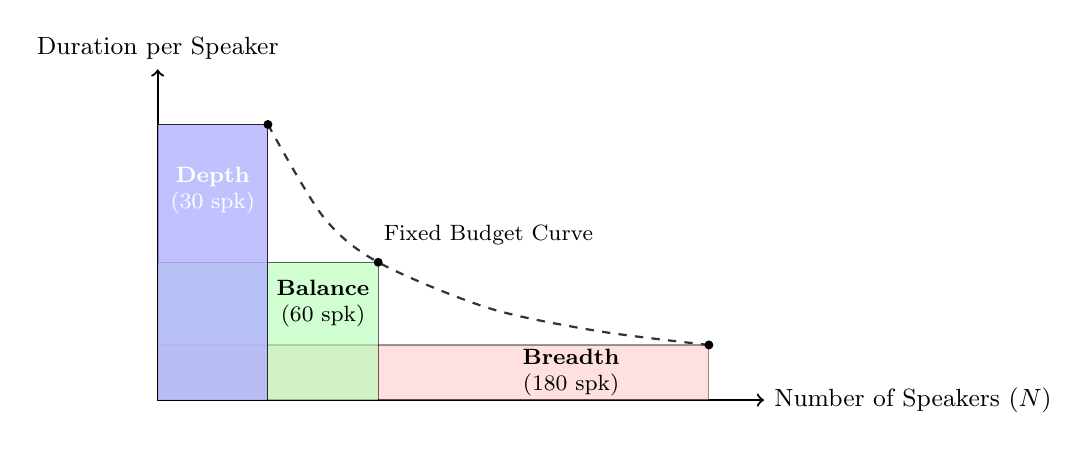
\begin{tikzpicture}[scale=0.7]
            % Axes
            \draw[->, thick] (0,0) -- (11,0) node[right] {\small Number of Speakers ($N$)};
            \draw[->, thick] (0,0) -- (0,6) node[above] {\small Duration per Speaker};

            % Breadth (Wide and Short)
            \draw[fill=red!30, opacity=0.4] (0,0) rectangle (10, 1);
            \node[align=center, font=\footnotesize] at (7.5, 0.5) {\textbf{Breadth}\\(180 spk)};

            % Balance (Medium)
            \draw[fill=green!30, opacity=0.6] (0,0) rectangle (4, 2.5);
            \node[align=center, font=\footnotesize] at (3, 1.75) {\textbf{Balance}\\(60 spk)};

            % Depth (Tall and Narrow)
            \draw[fill=blue!30, opacity=0.8] (0,0) rectangle (2, 5);
            \node[align=center, font=\footnotesize, text=white] at (1, 3.8) {\textbf{Depth}\\(30 spk)};

            % Instead of a straight line, we use a smooth curve connecting the corners
            % Corners are at: (2,5), (4,2.5), (10,1)
            \draw[dashed, thick, black!80] plot [smooth] coordinates {(2,5) (3,3.33) (4,2.5) (6,1.67) (8,1.25) (10,1)};

            % Label for the line
            \node[fill=white, inner sep=2pt, font=\footnotesize, sloped] at (6, 3) {Fixed Budget Curve};

            % Optional: Dots at the intersection points to emphasize them
            \filldraw (2,5) circle (2pt);
            \filldraw (4,2.5) circle (2pt);
            \filldraw (10,1) circle (2pt);
      \end{tikzpicture}
      \caption{Visual representation of the data strategies. The area of each rectangle (Total Audio) remains constant ($\approx 22.5 hours$), illustrating the trade-off between speaker diversity (Breadth) and data density (Depth).}\label{fig:data_strategy}
\end{figure}

Only speakers with at least the required minimum duration for the specific
subset were eligible for selection (e.g., at least 45 minutes for the
30-speaker set).

To ensure fair evaluation, speaker sets were nested: the 30 speakers in the
30-speaker set are included in the 60-speaker set, which are included in the
180-speaker set. An exact 50/50 male-female split was maintained in all
datasets to avoid gender bias.

This decision will allow using the same speakers for evaluation across all
models.

\subsection{Preprocessing}

\subsubsection{Text Normalization and Accentuation}

Raw Liepa~2 transcripts are largely normalized (numbers, dates, abbreviations,
and acronyms are expanded), however, some additional normalization was required
to standardize the text for grapheme-based TTS training:

\begin{enumerate}
      \item \textbf{Cleaning:} Rare and non-standard punctuation was mapped to a standard set (.,-?!) and remaining extraneous characters were removed.
      \item \textbf{Whitespace:} Consecutive whitespace characters were collapsed, and leading/trailing whitespace was trimmed.
      \item \textbf{Accentuation:} Raw text was processed using \textbf{Kirčiuoklis}~\cite{kirciuoklis} for automatic stress assignment. Ambiguous homographs were left unaccentuated, relying on the model to infer prosody from context.
      \item \textbf{Lowercasing:} All text was converted to lowercase to reduce the vocabulary size.
      \item \textbf{Letter substitution:} Non-Lithuanian letters were replaced with equivalents (`q' $\to$ `k', `w' $\to$ `v', `x' $\to$ `ks').
\end{enumerate}

As a result of these normalization steps, the vocabulary size is reduced from
140~characters to 41~characters. The final alphabet used for training consists
of the following characters:
\begin{center}
      \texttt{a ą b c č d e ę ė f g h i į y j k l m n o p r s š t u ų ū v z ž ´ ` \textasciitilde{} (space) . , - ? !}
\end{center}

\subsubsection{Audio Preprocessing}

Audio recordings were resampled from their original \textbf{16,000 Hz} to
\textbf{22,050 Hz}. While resampling to a higher frequency does not add new
information, the resampling was performed to match the pre-trained vocoder.
Leading and trailing silence was trimmed. Acoustic features were extracted
using the parameters in~\ref{tab:audio_params}

\begin{table}[htbp]
      \centering
      \caption{Mel-spectrogram extraction parameters.}\label{tab:audio_params}
      \begin{tabular}{lr}
            \toprule
            \textbf{Parameter} & \textbf{Value}        \\
            \midrule
            Sampling Rate      & 22,050 Hz             \\
            FFT Size           & 1024 samples (46 ms)  \\
            Hop Length         & 256 samples (11.6 ms) \\
            Window Length      & 1024                  \\
            Mel Channels       & 80                    \\
            Frequency Range    & 0--8000 Hz            \\
            Pre-emphasis       & 0.98                  \\
            \bottomrule
      \end{tabular}
\end{table}

A complete list of audio parameters is presented in the
Appendix~\ref{appendix:audio_params}

\subsection{Model Architectures}

Models were implemented using the \textbf{Coqui TTS}~\cite{coqui2021}
framework.

\subsubsection{Speaker Conditioning}

To enable multi-speaker synthesis, speaker identity was provided via
fixed-length embeddings, specifically \textbf{x-vectors}~\cite{snyder2018x}.
These 512-dimensional were extracted using a speaker
encoder~\cite{jia2019transfer} pre-trained on VoxCeleb (available in the Coqui
TTS model zoo) and kept frozen during TTS model training.

\textbf{Tacotron~2} used both the external x-vectors (concatenated to
encoder output) and a learnable embedding layer.

\textbf{Glow-TTS} used only learnable fixed-length speaker embeddings since the Glow-TTS implementation does not support both types simultaneously.

\subsubsection{Tacotron~2 (Autoregressive)}

The autoregressive model used is \textbf{Tacotron~2}, modified with Dynamic
Convolutional Attention (DCA) to accelerate alignment convergence.

\begin{itemize}
      \item \textbf{Encoder:} 3-layer convolutional stack + bi-directional LSTM (512 units).
      \item \textbf{Decoder:} 2-layer LSTM (1024 units) with location-sensitive attention.
\end{itemize}

The training objective $\mathcal{L}_{T2}$ is a weighted sum of auxiliary
losses:
\begin{equation}
      \mathcal{L}_{T2} = \mathcal{L}_{L1} + \mathcal{L}_{Post} + \lambda_{SSIM}(\mathcal{L}_{SSIM}) + \lambda_{attn}(\mathcal{L}_{Guided}) + \lambda_{stop}(\mathcal{L}_{Stop})
\end{equation}
Where $\mathcal{L}_{Guided}$ enforces diagonal attention alignment, critical for long-form synthesis.

\subsubsection{Glow-TTS (Non-autoregressive)}

The non-autoregressive model is \textbf{Glow-TTS}, a flow-based architecture
with MAS.

\begin{itemize}
      \item \textbf{Backbone:} Transformer encoder and flow-based decoder.
      \item \textbf{Alignment:} Trained using unsupervised Soft-DTW (Dynamic Time Warping) to generate duration targets without external aligners.
      \item \textbf{Predictors:} Explicit 1D-convolutional duration predictor.
\end{itemize}

The objective function is the exact log-likelihood of the data:
\begin{equation}
      \log P_X(x|c) = \sum_{j=1}^{T_{mel}} \log \left| \det \frac{\partial z_j}{\partial x_j} \right| + \sum_{j=1}^{T_{mel}} \log \mathcal{N}(z_j; \mu, \sigma)
\end{equation}
Additionally, a duration predictor is trained via MSE loss $\mathcal{L}_{dur}$ to predict phoneme durations.

\subsubsection{Vocoder}

A \textbf{HiFi-GAN v2}~\cite{kong2020hifi} model, pre-trained on the
multi-speaker VCTK corpus~\cite{veaux2019cstr}, was used as the vocoder for all
acoustic models. All weights were frozen to isolate the performance differences
to the acoustic models only.

\subsection{Model Training Configurations}

\subsubsection{Environment and Framework}

Experiments were conducted on a personal workstation equipped with an AMD Epyc
7642 CPU, 256 GB RAM, and NVIDIA GeForce RTX 3090 (24 GB) GPU\@. The software
environment included Ubuntu 25.04, Python 3.13.3, Coqui TTS v0.27.2, and CUDA
13.0 for GPU acceleration. The pipeline was automated via Make, with separate
steps for data preprocessing, speaker embedding computation, model training,
inference, and synthesized sample deployment to the evaluation web app.

The exact Python environment configuration is provided in the accompanying
GitHub repository, file \texttt{pyproject.toml}.

In the TTS training stage, the validation loss was evaluated every epoch
($\approx$ 450 steps) using a held-out 1\% validation split. The best model
checkpoint was selected based on the lowest validation loss.

\subsubsection{Tacotron~2 Configuration}

The Tacotron~2 model was trained using the Dynamic Convolution Attention (DCA)
mechanism to improve alignment stability.

The model optimization utilized a composite loss function consisting of Decoder
L1 loss ($\alpha=0.25$), Post-net L1 loss ($\alpha=0.25$), Decoder and Post-net
SSIM losses ($\alpha=0.25$ each), Guided Attention loss ($\alpha=5.0$), and a
weighted Stop token loss (weight=$15.0$).

Notably, the default NoamLR learning rate scheduler caused high gradient
values, instability, and sub-optimal convergence for Tacotron~2. Therefore, a
MultiStepLR scheduler with more aggressive decay of 0.5 every 10,000 steps was
used instead after empirical testing. The main hyperparameters are shown
in~\ref{tab:tacotron_config}

\begin{table}[h!]
      \centering
      \caption{Tacotron~2 DCA training configuration.}\label{tab:tacotron_config}
      \begin{tabular}{lr}
            \toprule
            \textbf{Parameter}    & \textbf{Value}                                        \\
            \midrule
            Validation split      & 1\%                                                   \\
            Batch size            & 64                                                    \\
            Initial Learning Rate & 0.0005                                                \\
            Optimizer             & RAdam                                                 \\
            LR schedule           & MultiStepLR (Decay 0.5 at steps 20k, 30k, \dots, 70k) \\
            Max epochs            & 200 ($\approx$ 90,000 steps)                          \\
            Attention type        & Dynamic Convolution                                   \\
            Separate stopnet      & True                                                  \\
            Speaker embedding dim & 512                                                   \\
            Number of speakers    & 30 / 60 / 180                                         \\
            \bottomrule
      \end{tabular}
\end{table}

\subsubsection{Glow-TTS Configuration}

The Glow-TTS was trained using Negative Log-Likelihood (NLL) for the flow
decoder and a monotonic alignment search. Unlike Tacotron~2, Glow-TTS converged
stably with the NoamLR scheduler, but required a higher number of epochs for
convergence. The configuration is shown in~\ref{tab:glow_config}

\begin{table}[h!]
      \centering
      \caption{Glow-TTS training configuration.}\label{tab:glow_config}
      \begin{tabular}{lr}
            \toprule
            \textbf{Parameter}       & \textbf{Value}                \\
            \midrule
            Validation split         & 1\%                           \\
            Batch size               & 64                            \\
            Maximum Learning Rate    & 0.001                         \\
            Optimizer                & RAdam                         \\
            LR scheduler             & NoamLR                        \\
            Warmup steps             & 4000                          \\
            Max epochs               & 400 ($\approx$ 180,000 steps) \\
            Encoder type             & Rel. Pos. Transformer         \\
            Encoder layers           & 6                             \\
            Encoder heads            & 2                             \\
            Encoder hidden dim       & 192                           \\
            Decoder hidden dim       & 192                           \\
            Decoder flow blocks      & 12                            \\
            Decoder block layers     & 4                             \\
            Mel-spectrogram channels & 80                            \\
            Speaker embedding dim    & 512                           \\
            Number of speakers       & 30 / 60 / 180                 \\
            \bottomrule
      \end{tabular}
\end{table}

The loss function was a combination of Negative Log-Likelihood (NLL) loss for
the flow-based decoder, Duration loss (MSE).

\subsection{Evaluation Protocol}

The synthesized speech from the trained models was evaluated using a
combination of objective and subjective metrics.

\subsubsection{Objective Evaluation}

A held-out test set of 60 standardized sentences (using seen speakers) was used
to calculate acoustic metrics. While useful for monitoring training, these
metrics do not perfectly correlate with human perception and served primarily
as diagnostic tools.

\begin{itemize}
      \item \textbf{MCD:} Spectral distance between synthesized and ground truth Mel-spectrograms.
      \item \textbf{F0~RMSE:} Root Mean Square Error between predicted and ground truth fundamental frequency (F0) contours.
      \item \textbf{Attention Alignment:} The \textbf{attention alignment plots} were generated during every epoch, and inspected regularly. A failure to converge to a diagonal alignment indicates that the model has failed to learn the text-to-audio mapping. This is especially relevant for the 180-speaker scenario to detect convergence failures caused by data sparsity.
\end{itemize}

\subsubsection{Subjective Evaluation (MOS)}

Naturalness was evaluated via a web-based listening test employing a
\textbf{Latin square design} to mitigate order and repetition biases. The
application was developed specifically for this study, and the source code is
available in the accompanying GitHub repository, folder
\texttt{tts\_rating\_app}.

The participants were 21 native Lithuanian speakers recruited through
university networks and social media platforms. Each rater evaluated a
randomized block of sentences, ensuring balanced exposure to all models and
sentences.

Naturalness was rated using the standard 5-point MOS scale. The test samples
were generated using the 6 experimental models plus a human ground truth,
evaluated on the same set of 60 held-out test sentences uttered by 6 speakers
(3 male, 3 female, 10 sentences each) randomly selected from the 30-speaker
subset.

%%%%%%%%%%%%%%%%%%%%%%%%%%%%%%%%%%%%%%%%%%%%%%%%%%%%%%%%%%%%%%%%%%%%%%%%%%%%%%%%
%% Results and analysis
%%%%%%%%%%%%%%%%%%%%%%%%%%%%%%%%%%%%%%%%%%%%%%%%%%%%%%%%%%%%%%%%%%%%%%%%%%%%%%%%
\section{Results and Analysis}

This chapter presents the quantitative and qualitative findings of the study.
The performance of the autoregressive (Tacotron~2) and non-autoregressive
(Glow-TTS) models is analyzed across the three data subsets defined in
Chapter~3: 30 speakers (45 minutes per speaker), 60 speakers (22.5 minutes per
speaker), and 180 speakers (7.5 minutes per speaker).

\subsection{Objective Evaluation}

Objective metrics provide insight into the acoustic accuracy and convergence
stability of the models.

Mel-Cepstral Distortion quantifies spectral fidelity, and is calculated as:
\begin{equation}
      \text{MCD} = \frac{10}{\ln 10} \times \sqrt{2 \sum_{n=1}^{K} (mc_n^{(syn)} - mc_n^{(gt)})^2}
\end{equation}
Where $mc_n^{(syn)}$ and $mc_n^{(gt)}$ are the $n$-th mel-cepstral coefficients of
the synthesized and ground truth speech, respectively, and $K$ is the number of
coefficients (here: 24).

F0~RMSE measures pitch accuracy:
\begin{equation}
      \text{F0~RMSE} = \sqrt{\frac{1}{T}\sum_{t=1}^{T} (F0_t^{(syn)} - F0_t^{(gt)})^2}
\end{equation}
Where $F0_t^{(syn)}$ and $F0_t^{(gt)}$ are the fundamental frequency values at time $t$ for
synthesized and ground truth speech, respectively, and $T$ is the total number of frames.

Since the original and synthesized audio may differ in length due to alignment
variations, Dynamic Time Warping (DTW) is applied to align the Mel-spectrograms
and F0 contours before computing MCD and F0~RMSE\@.

\ref{tab:objective_results} summarizes the MCD and F0~RMSE on the
held-out test set.

\begin{table}[htbp]
      \centering
      \caption{Objective evaluation results. Lower is better. \textbf{Bold} indicates best performance per architecture.}\label{tab:objective_results}
      \begin{tabular}{llcc}
            \toprule
            \textbf{Model} & \textbf{Speaker Count ($N$)} & \textbf{MCD (dB)} & \textbf{F0~RMSE (Hz)} \\
            \midrule
            \multirow{3}{*}{Tacotron~2}
                           & 30                           & 9.58              & 31.28                 \\
                           & 60                           & \textbf{9.55}     & \textbf{30.49}        \\
                           & 180                          & 9.63              & 31.06                 \\
            \midrule
            \multirow{3}{*}{Glow-TTS}
                           & 30                           & \textbf{9.90}     & 37.86                 \\
                           & 60                           & 10.00             & 36.18                 \\
                           & 180                          & 9.98              & \textbf{35.69}        \\
            \bottomrule
      \end{tabular}
\end{table}

Across all data subsets, Tacotron~2 moderately, but consistently outperformed
Glow-TTS in pitch accuracy (F0~RMSE). Interestingly, both models showed
remarkable insensitivity to the data composition strategy in terms of objective
metrics, with only minor variations observed --- the intra-model differences
were relatively small for MCD (within 0.1 dB) and for F0~RMSE (within 3 Hz).
The 180-speaker configuration outperformed the other two in F0~RMSE for
Glow-TTS, suggesting that increased speaker diversity did not harm pitch
modeling, and may have even helped generalization.

\subsubsection{Alignment Convergence}

Alignment stability during training was monitored via attention alignment
plots, provided by the TensorBoard integration in Coqui TTS\@.

\textbf{Tacotron~2} demonstrated no visible sensitivity to data sparsity. On all subsets, the attention mechanism converged to a clear diagonal alignment within 10k steps. While there were occasional minor misalignments during training, by the end of training, all models exhibited stable alignments on all test sentences.

As seen in Figure, the attention maps for Tacotron~2 remain stable across all
data subsets, indicating robust alignment learning even in low-resource
conditions.

% FIXME ~\ref{fig:alignments}

\textbf{Glow-TTS}, utilizing MAS, also converged successfully across all three subsets. However, despite robust alignment, the audio reconstruction quality was significantly lower than Tacotron~2.

\subsubsection{Pitch and Spectral Accuracy}

Tacotron~2 consistently outperformed Glow-TTS in pitch accuracy (F0~RMSE),
achieving values around 31~Hz compared to Glow-TTS's 36~Hz. Furthermore,
Tacotron~2 achieved slightly lower MCD scores on all subsets, suggesting it
captures fine-grained spectral details better than the flow-based decoder. The
raters noted that Glow-TTS outputs often sounded monotone and robotic, possibly
due to Glow-TTS not having an explicit pitch predictor.

Spectral analysis confirms the objective metrics. As illustrated in the
spectrogram comparison, Tacotron~2 captures visibly more fine-grained spectral
details and intonation contours more accurately than Glow-TTS, which tends to
produce flatter, less dynamic outputs.

% TODO \ref{fig:spectrogram_comparison},

\subsection{Subjective Evaluation (MOS)}

Naturalness was evaluated via a Latin square design listening test with 21
native speakers, who rated samples from all six experimental models plus the
ground truth on a 5-point MOS scale. The results are presented
in~\ref{tab:mos_results}

\begin{table}[htbp]
      \centering
      \caption{5-point MOS results with 95\% Confidence Intervals.}\label{tab:mos_results}
      \begin{tabular}{llc}
            \toprule
            \textbf{Model}        & \textbf{Speaker count ($N$)} & \textbf{MOS (95\% CI)}   \\
            \midrule
            \textbf{Ground Truth} & ---                          & \textbf{4.89} $\pm$ 0.xx \\
            \midrule
            \multirow{3}{*}{Tacotron~2}
                                  & 30                           & 3.39 $\pm$ 0.xx          \\
                                  & 60                           & \textbf{3.48} $\pm$ 0.xx \\
                                  & 180                          & 3.27 $\pm$ 0.xx          \\
            \midrule
            \multirow{3}{*}{Glow-TTS}
                                  & 30                           & 2.40 $\pm$ 0.xx          \\
                                  & 60                           & 2.39 $\pm$ 0.xx          \\
                                  & 180                          & 2.16 $\pm$ 0.xx          \\
            \bottomrule
      \end{tabular}
\end{table}

These results are in line with the objective findings --- Tacotron~2
outperforms Glow-TTS in naturalness across all data strategies. Additionally,
Tacotron~2's performance peaks in the 60-speaker configuration. Here, too,
these models exhibit little sensitivity to data composition in terms of MOS\@.

\subsubsection{Architecture Comparison}

The MOS results reveal a significant performance gap between the two
architectures.

\textbf{Tacotron~2} achieved the highest synthesis quality in the study, with the 60-speaker configuration scoring $3.48$. Listeners noted that when Tacotron~2 works, it produces highly expressive prosody. Increasing the speaker count to 180 caused a moderate drop in naturalness to $3.27$.

\textbf{Glow-TTS} lagged behind Tacotron~2 in naturalness, with MOS scores around $2.2$--$2.4$. The listeners reported that Glow-TTS seemed to have strong robotic artifacts, and was at times unintelligible. This was especially pronounced in the 180-speaker condition where the MOS dropped to $2.16$.

\subsubsection{Optimal Composition}

There was no clear winner between the data strategies across both
architectures. The 60-speaker configuration held a slight edge for Tacotron~2,
while the 30-speaker configuration was marginally (insignificantly) better for
Glow-TTS\@. However, both models performed worst in the 180-speaker scenario,
indicating that excessive speaker diversity with minimal data per speaker
hinders synthesis quality.

\subsubsection{Speaker Analysis}

An analysis of individual speakers' MOS scores was conducted to identify any
patterns related to speaker identity. \ref{tab:speaker_mos} summarizes the
average MOS per speaker across all models.

\begin{table}[ht]
      \centering
      \caption{Average MOS per speaker across all models.}\label{tab:speaker_mos}
      \begin{tabular}{lcc}
            \toprule
            \textbf{Speaker ID} & \textbf{Tacotron~2 MOS}   & \textbf{Glow-TTS MOS} \\
            \midrule
            AS009               & \underline{\textbf{4.42}} & \textbf{2.95}         \\
            IS031               & 3.45                      & 2.43                  \\
            IS038               & 3.95                      & 2.80                  \\
            MS052               & 2.36                      & 2.03                  \\
            VP131               & 2.70                      & 2.04                  \\
            VP427               & 3.37                      & 1.60                  \\
            \bottomrule
      \end{tabular}
\end{table}

Notably, speaker AS009 consistently received the highest ratings across both
models, suggesting that certain speaker or dataset characteristics (e.g., clear
articulation, consistent recording quality, or clean transcripts) may
facilitate better synthesis quality. On the other hand, speakers like MS052 and
VP427 scored lower, indicating potential data quality issues or inherent
speaker traits (e.g., strong accents, background noise) that challenge the TTS
models.

\subsection{Discussion}

The results provide the following key insights:

% \begin{enumerate}
%       \item \textbf{Performance gap:} Tacotron~2 strictly outperformed Glow-TTS in both objective (RMSE, MCD) and subjective (MOS) metrics across all data strategies. The 180-speaker scenario caused a slight to moderate quality drop for both models, but Tacotron~2 was able to produce intelligible speech.
%       \item \textbf{Architectural suitability:} While non-autoregressive models like Glow-TTS are theoretically more robust to alignment errors, in this specific implementation and dataset, the autoregressive Tacotron~2 yielded significantly higher naturalness.
%       \item \textbf{The ``Balance'' Sweet Spot:} The superior performance of the 60-speaker configuration indicates that for a fixed budget of 22.5 hours, 60 speakers provide a better regularization effect than 30 speakers, preventing overfitting while providing enough data to stabilize the attention mechanism.
% \end{enumerate}

%%%%%%%%%%%%%%%%%%%%%%%%%%%%%%%%%%%%%%%%%%%%%%%%%%%%%%%%%%%%%%%%%%%%%%%%%%%%%%%%
%% Conclusion
%%%%%%%%%%%%%%%%%%%%%%%%%%%%%%%%%%%%%%%%%%%%%%%%%%%%%%%%%%%%%%%%%%%%%%%%%%%%%%%%
\section{Conclusion}

\subsection{Summary of findings}

\subsection{Contributions}

\subsection{Limitations of the study}

\subsection{Future work}

%%%%%%%%%%%%%%%%%%%%%%%%%%%%%%%%%%%%%%%%%%%%%%%%%%%%%%%%%%%%%%%%%%%%%%%%%%%%%%%%
%% References
%%%%%%%%%%%%%%%%%%%%%%%%%%%%%%%%%%%%%%%%%%%%%%%%%%%%%%%%%%%%%%%%%%%%%%%%%%%%%%%%
\section{\phantom{Appendix} References}

\printbibliography[heading=none]

% Examples are also provided for ChatGPT citation, both in general~\cite{chatgpt_bendrai} and for a specific conversation~\cite{chatgpt_pokalbis}.

\section{\phantom{Appendix} Appendix: Audio preprocessing parameters}\label{appendix:audio_params}

The following Mel-spectrogram extraction parameters were used by all models
(Tacotron~2, Glow-TTS, and HiFi-GAN~v2 vocoder):

\begin{table}[ht]
      \centering
      \caption{Complete Mel-spectrogram extraction parameters.}\label{tab:audio_params_full}
      \begin{tabular}{lr}
            \toprule
            \textbf{Parameter}      & \textbf{Value} \\
            \midrule
            fft\_size               & 1024           \\
            win\_length             & 1024           \\
            hop\_length             & 256            \\
            frame\_length\_ms       & null           \\
            frame\_shift\_ms        & null           \\
            stft\_pad\_mode         & ``reflect''    \\
            sample\_rate            & 22050          \\
            resample                & false          \\
            preemphasis             & 0.98           \\
            ref\_level\_db          & 20             \\
            do\_sound\_norm         & false          \\
            log\_func               & ``np.log10''   \\
            do\_trim\_silence       & true           \\
            trim\_db                & 60             \\
            do\_rms\_norm           & false          \\
            db\_level               & null           \\
            power                   & 1.5            \\
            griffin\_lim\_iters     & 60             \\
            num\_mels               & 80             \\
            mel\_fmin               & 0.0            \\
            mel\_fmax               & 8000.0         \\
            spec\_gain              & 20             \\
            do\_amp\_to\_db\_linear & true           \\
            do\_amp\_to\_db\_mel    & true           \\
            pitch\_fmax             & 640.0          \\
            pitch\_fmin             & 1.0            \\
            signal\_norm            & true           \\
            min\_level\_db          & -100           \\
            symmetric\_norm         & true           \\
            max\_norm               & 4.0            \\
            clip\_norm              & true           \\
            stats\_path             & null           \\
            \bottomrule
      \end{tabular}
\end{table}

\end{document}
